\chapter{Introduction}\label{sec:introduction}

This thesis focuses on the application of Operational Research (OR) to
healthcare systems and in
particular at the interface of Emergency Departments (EDs) and Emergency
Medical Services (EMS).
OR models have been used a lot in the past in conjunction with healthcare
systems to better inform the decision-making of healthcare managers and
policy makers.
The use of OR in healthcare systems can be particularly useful in situations
where improvements in the system are needed to cope with the demand for
healthcare services.

OR is a field of study that makes use of mathematical
and computational techniques to solve problems in a wide range of areas, such
as healthcare, business, engineering, and the military.
The core of OR has been to help decision makers make better decisions by
providing them with the tools to analyse and understand the problem at hand and
the possible solutions to it.
Such mathematical tools include queueing theory, game theory, decision theory,
statistical analysis, machine learning and many more.

This research was funded by The Healthcare Improvement Studies (THIS) Institute
of the University of Cambridge.
The THIS Institute is a research institute that aims to create a world-leading
scientific asset for the National Health Service (NHS) about how to improve
quality and safety in healthcare.

The introductory Chapter is structured in the following way:
\begin{itemize}
    \item Section~\ref{sec:intro_or_history} provides an overview of the
    history of OR and its development, along with a brief introduction to
    queueing theory and game theory.
    \item Section~\ref{sec:intro_healthcare_congestion} introduces the problem
    of congestion in healthcare systems and in particular in EDs.
    \item Section~\ref{sec:intro_research} presents the research questions and
    objectives of this thesis, along with the overall structure of the thesis.
    \item Section~\ref{sec:intro_software} provides an overview of the software
    development tools and best practices that were used in this research.
\end{itemize}


\section{History of Operational Research}\label{sec:intro_or_history}

The history of OR can be traced back to the 1940s during Would War II when the
UK forces started to use OR techniques to optimise the use of their aircrafts.
Patrick Blackett was a British physicist and a mathematician and was one of the
first people to use OR techniques to solve problems in the military and was
later referred to as the \textit{father of OR}~\cite{blackett1962studies}.
At the time, many strategic problems were too complicated to solve by any one
person or a single discipline.
Scientists and mathematicians from different fields were brought together to
solve problems such as finding the best strategies of air defence, minimising
losses from submarines and radar deployment.
These teams were called \textit{Operational Research teams} or
\textit{Operations Research teams} and the collection of techniques that they
used were later used to form the discipline of
OR~\cite{ravindran2008operations}.

After the war, the discipline of OR started to grow and spread to other
industries and fields.
Universities started advancing the field by developing new techniques and
methods and later started to offer undergraduate and postgraduate courses on it.
Additionally, the introduction of electronic computers allowed OR techniques to
be used in more complex problems~\cite{ravindran2008operations}.
The first formal definition of OR was given by the British Operational
Research Society:

\begin{quotation}
    ``Operational research is the application of the methods of science to
    complex problems arising in the direction and management of large systems of
    % <!-- alex ignore gals-man -->
    men, machines, materials and money in industry, business, government, and
    defence.
    The distinctive approach is to develop a scientific model of the system,
    incorporating measurement of factors such as chance and risk, with which to
    predict and compare the outcomes of alternative decisions, strategies or
    controls.
    The purpose is to help management determine its policy and actions
    scientifically''~\cite{or_for_multi_organizations}.
\end{quotation}

There are numerous methods and techniques that form the discipline of OR.
Some of the most common ones are mathematical programming, queueing theory,
game theory, decision theory, data mining and statistical analysis.
The main OR techniques that are used in this thesis are queueing theoretic
models and game theoretic models.

Queueing theory is a branch of OR that studies queues like those found in
banks, supermarkets, hospitals and many more.
A queueing model is an abstract representation of a system whose purpose is
to understand the underlying behaviour of the system so that informed and
intelligent decisions can be made.
Queuing theory was first introduced in 1909 by A.K. Erlang, who was a Danish
mathematician and engineer, where it was applied to the problem of
telecommunications~\cite{erlang1909}.
Erlang placed the foundation for the Poisson distribution in queueing theory
which then led to the development of the Exponential distribution.
The motivation for the work around queueing theory between \(1920\) and
\(1930\) has been the practical problem of congestion.
In the early \(1950\)s applications of queueing theory started to develop
outside the field of telecommunications and in \(1960\)s queueing theory
was utilised for the performance evaluation of computer systems.
Ever since, queueing theory and its applications have been growing and
expanding to many different areas~\cite{sztrik2010queueing}.

Another branch of OR that is used in this thesis is game theory.
Game theory focuses on the study of strategic interaction between players and
the outcomes of such interactions.
It is widely used to study behavioural patterns of players in a game and
explore strategies that players can use to maximise their payoff.
Although mathematicians have been studying strategic games for a long time now,
it was not until \(1940\)s that game theory started receiving more attention
with the publication of John von Neumann and Oskar
Morgenstern~\cite{von1947theory}.
The book introduced the mathematical theory of economic and social organisation,
based on a theory of games of strategy.
Around \(1950\), mathematician John Nash developed a criterion for mutual
consistency of players' strategies, which is a concept now known as the
\textit{Nash equilibrium}.
Nash proved that for every finite \(n\)-player, non-cooperative game there
exists a Nash equilibrium in mixed strategies.
In the next few decades, game theory started to be applied to many different
areas such as economics, biology, politics, psychology and many more.
In the last few years, game theory has also been applied to healthcare
systems~\cite{koutsoupias1999worst, TwoTierHealthcareSystem}.



\section{Congestion in healthcare}\label{sec:intro_healthcare_congestion}

EDs are one of the most important parts of a hospital and are the first point
of contact for individuals seeking medical attention.
It is also one of the most congested areas of a hospital and is often the
cause of long waiting times for patients.
EDs are under increasing pressure to meet patient waiting time targets and
satisfy regulation targets~\cite{EmergencyDepartmentWinterPressures}.
It is widely reported that ED congestion severely impacts not only patients in
the ED but also the EMS~\cite{mirror, bmj, thenews}.
One of the major concern for the ambulance service is that the ambulances are
held waiting parked outside the EDs to offload (dispatch) their patients when
the ED is particularly busy~\cite{clarey2014ambulance}.
As a result, ambulance blocking not only impacts patients that are waiting for
ED service, but has a major knock-on effect on the ability of ambulances to
respond to new EMS calls, and thus placing lives at risk~\cite{eastanglia}.

There are numerous news articles that address the complications that arise when
ambulances stay blocked outside of hospitals for a long amount of
time~\cite{dailyrecords, staffordshirelive}.
Most such news reports comment on the long idle time of ambulances when
being blocked outside of hospitals and not being utilised as best as they
could be~\cite{herefordtimes}.
In addition, there are several reports of examples where this became an issue
for new patients that needed to be transported to a hospital but were unable
to do so due to the ambulance taking too long to reach
them~\cite{southwalesargus}.
Some even mention the negative effect that this has on the morale of ambulance
paramedics~\cite{bbcwales}.

In the United Kingdom, the NHS sets some regulations on ED performance.
One of these regulations is that 95\% of patients that arrive at the ED should
be admitted, transferred or discharged within four hours.
This is where gaming behaviour might be observed between the EDs and the EMS.



\section{Research questions and thesis structure}\label{sec:intro_research}


This thesis aims to explore behavioural patterns that emerge at the ED-EMS
interface using a game theoretic model that is informed by an underlying
queueing network.
A model is developed that describes the situation where an ambulance service
would have to distribute its patients between two EDs.
The two EDs are thought of as two queueing systems and the EMS as a distributor
that decides how to distribute patients to them, aiming to minimise some
performance measure.
The patients that are distributed by the EMS arrive at the EDs via an ambulance
and are then either offloaded at the ED or stay blocked outside in the
ambulance.
This is where gaming behaviour is incorporated into the model.
The managerial decision of whether or not to offload a patient is a strategic
decision that is made by the two EDs.
This decision is mapped to a parameter that will be referred to as the
\textit{threshold} of the ED.
A high threshold indicates that the ED accepts ambulance patients more often,
while a low threshold means that the ED blocks ambulances more frequently.
The model is then used to explore the emergent behaviour of the system.

The main research questions of the research presented in this thesis are:
\begin{itemize}
    \item How can queueing theory be used to model an Emergency Department that
    can accept and block patients from an ambulance service?
    \item How can one extract performance measures from such a queueing model?
    \item How can game theory be used to model the interaction between the EMS
    and two EDs?
    \item How can the developed model be used to explore the emergent behaviour
    of the system?
    \item How can agent-based modelling be used to model how staff at the EDs
    may choose the speed at which they serve patients in order to maximise some
    utility.
\end{itemize}

Specifically, the focus is on the construction of a 3-player game theoretic
model between two queueing systems and a service that distributes individuals
to them.
The resultant model is used to explore the emergent dynamics between the three
players.
This study explores two new concepts: obtaining performance measures for a new
queueing theoretic model with a service centre and a buffer space and, and
using a learning algorithm to model the emergence of behaviour.
The developed theoretical model is illustrated through the application to
a healthcare system of two EDs and the EMS, exploring the inefficiencies that
emerge and ways to apply some incentive mechanisms to improve them.
The EDs are modelled as two queueing systems each with a tandem buffer and a
service centre.
The performance measures are then used as the utilities of the game.
The novelty of the queueing model here is a contribution not only to game
theoretic literature but also to the queueing theoretic literature, since
no such model of a tandem queueing model with a pair of parameters for the
buffer has been previously considered.

This thesis aims to explore the behaviour that emerges from an interactive
situation between two queueing systems that aim to maximise their own utility.
In addition, this research focuses on the impact that this may have on the
ambulance's blocking time and patients' waiting time.

The research presented on this thesis is based on the following assumptions:
\begin{itemize}
    \item Some managerial decision making is involved in choosing when to start
    the blockage of ambulances.
    \item The ambulance service decides how patients are distributed to
    different hospitals rather than choosing the nearest hospital for each
    patient.
    \item The waiting time of a patient, arriving by an ambulance in the ED, is
    measured from the time they are offloaded to the ED itself, rather than
    from the time the ambulance arrives at the parking space.
\end{itemize}

The research presented in this thesis consists of four main chapters.
That is a chapter on the queueing theory model that is presented introduced
in this thesis, a chapter on the game theoretic model that uses the queueing
model in its construction, a chapter on the numerical results of the game
theoretic model and a chapter on the agent-based model that is used to
explore some additional emergence of behaviour.
Overall, the thesis is structured as follows:
\begin{itemize}
    \item Chapter~\ref{sec:introduction} introduces the problem and
    motivation behind the research presented in this thesis.
    A background of OR as well as an overview of the
    software development process and best practices are also presented.
    \item Chapter~\ref{sec:lit_review} presents a literature review of the
    relevant research.
    This includes a review of the literature on OR models
    applied to healthcare systems, a review of the conjunction of queueing
    theory and game theory and a review of the literature on game theoretic
    models applied to healthcare systems.
    Moreover, a brief review on behavioural OR is also presented to provide
    some context for the agent-based model that is presented in this thesis.
    \item Chapter~\ref{sec:queueing_section} introduces a queueing network
    model that accepts two types of individuals and has two waiting spaces.
    Two modelling approaches are discussed; Discrete Event Simulation (DES) and
    the Markov chain (MC) approach.
    The chapter mainly focuses on the MC approach and presents how the steady
    state probabilities and certain performance measures can be obtained
    from it.
    This system is then used to describe an ED that accepts patients arriving
    by ambulance and patients that arrive by other means.
    \item Chapter~\ref{sec:game_theoretic_model} presents a game theoretic
    model that is informed by the queueing network model.
    The chapter starts by giving a brief overview of game theoretic concepts
    that are utilised in this chapter.
    The formulation of the game theoretic model is then presented along with
    the methodology that was used to solve it.
    The model is then mapped to a 3-player game between the EMS and two EDs.
    \item Chapter~\ref{sec:numerical_results} presents an overview of the
    numerical results of the game theoretic model.
    The chapter gives an overview of the data collection process as well as a
    brief description of the data parameters explored.
    The results of the numerical experiments are then presented and discussed.
    \item Chapter~\ref{sec:agent_based_extension} presents an extension to the
    queueing model discussed in Chapter~\ref{sec:queueing_section}.
    The queueing model is extended to use state-dependent and server-dependent
    service times instead of the constant service times that were previously
    used.
    An agent-based model is constructed where there are different service
    times for each server and each state of the system.
    A reinforcement learning algorithm is then used to observe the learning
    that takes place when servers choose the speed at which they serve
    individuals in order to maximise some utility.
    \item Chapter~\ref{sec:conclusion} presents an overall summary of the
    research presented in this thesis.
    The chapter also lists the main contributions of this thesis and presents
    some suggestions for future work.
\end{itemize}




\section{Software development and best practices}\label{sec:intro_software}

Scientists and researchers are increasingly using software development tools to
conduct their research.
In fact the use of software is becoming so prevalent that it is now
considered a fundamental part of the scientific process.
Yet software is not always developed following practices that ensure its
reproducibility and sustainability.
The best practices discussed in this section promote better quality software,
which in turn improves the research's reproducibility and
reusability~\cite{jimenez2017four}.

Open Source Software (OSS) is software with source code that everyone can
access, modify and improve.
OSS improves accessibility, reproduction, transparency and innovation in
scientific research~\cite{mulgan2005wide}.
Moreover, OSS development encourages developer-user communities and builds
trust among users~\cite{mckiernan2016open}.

The following list is a summary of best practices as described
in~\cite{wilson2014best}:

\begin{enumerate}
    \item Write programs for people, not computers. \label{best_practice_1}
    \item Let the computer do the work. \label{best_practice_2}
    \item Make incremental changes. \label{best_practice_3}
    \item Don't repeat yourself (or others). \label{best_practice_4}
    \item Plan for mistakes. \label{best_practice_5}
    \item Optimise software only after it works correctly.
    \label{best_practice_6}
    \item Document design and purpose, not mechanics. \label{best_practice_7}
    \item Collaborate. \label{best_practice_8}
\end{enumerate}

This is not an exhaustive list of best practices, rather it is a list of
principles that can be used to guide the development of software.
Software tools that are used together with these principles are version control,
code reviews, automated testing, code formatting and documentation.
These principles were used to guide the development of the software that is
presented in this thesis.
These concepts are also discussed in more detail in the following sections.

This thesis relies heavily on the use of software.
All code written for this thesis is written in the open source programming
language Python~\cite{van1995python}.
In particular, all software developed for this thesis is publicly available on
GitHub and is licensed under the MIT license.
The MIT license is a permissive license that allows users to inspect, modify
and redistribute the software.
The repository for the software developed for this thesis has also been
archived using Zenodo~\cite{ambulance_game_github_repo}.


\subsection{Version control}

A \textit{version control system} (VCS) is a system that manages the evolution
of an ongoing object.
It records any changes made by the software developers and allows them to
revert to previous versions of the software.
The adoption of VCS has become widespread in software development and has
empowered software developers to work effectively and collaboratively on large
projects.

Version control usually consists of three main components: a repository, a
working directory and a staging area.
The \textit{repository} is the place where the software is stored.
The \textit{working directory} is the place where the software is being
developed.
The \textit{staging area} is the place where the changes made to the software
are stored before they are committed to the history of the
repository~\cite{blischak2016quick}.

There are two main types of VCS: centralized VCS and distributed VCS.
Centralized VCS is a VCS where all the software developers work with a single
central repository.
The central repository is the only place where the software is stored and
where all the changes are made.
The most commonly used centralized VCS is Subversion and CVS.
The distributed VCS is a VCS where all the software developers work with a
local copy of the software.
The local copy of the software is then synchronised with a central repository
where the changes are made~\cite{zolkifli2018version}.
Some examples of distributed VCS are Git, Mercurial and Bazaar.
For the purposes of this thesis, the distributed VCS
Git~\cite{spinellis2012git} is used.

Git is a distributed VCS that is used to track changes in source code during
software development.
There are a number of services that host online Git servers that can be used to
store Git repositories.
The importance of using a Git server is that it allows for collaboration and
makes, not only the code, but also the history of the code available to
everyone.
Some examples of Git servers are GitHub, GitLab and BitBucket.
For the purposes of this thesis, the Git server GitHub is used.

GitHub has several features that make it a good choice for hosting Git
repositories.
It is a web-based Git repository hosting service that allows users to
collaborate on projects.
Every new feature or bug fix that was developed for this thesis was developed
in a separate branch of the repository.
GitHub allows users to create branches that are used to develop features
independently of the main code base.
Once the feature is complete, the branch is merged into the main code base.
This process is called \textit{branching} and it is a core concept of Git.
Branching allows developers to work on multiple features at the same time and
to collaborate with other developers.
It also allows developers to work on a feature without affecting the main code
base.

GitHub also offers users the ability to comment on each other's code, to review
each other's code and raise issues on each other's repositories.
This is often done through a process called a \textit{pull request} (PR).
A PR is a mechanism for a developer to notify team members that they have
completed a feature.
The team members review the changes, discuss potential improvements and
eventually approve and merge the changes into the main code base.
Figure~\ref{fig:github_pr} shows an example of a PR on GitHub.

\begin{figure}[H]
    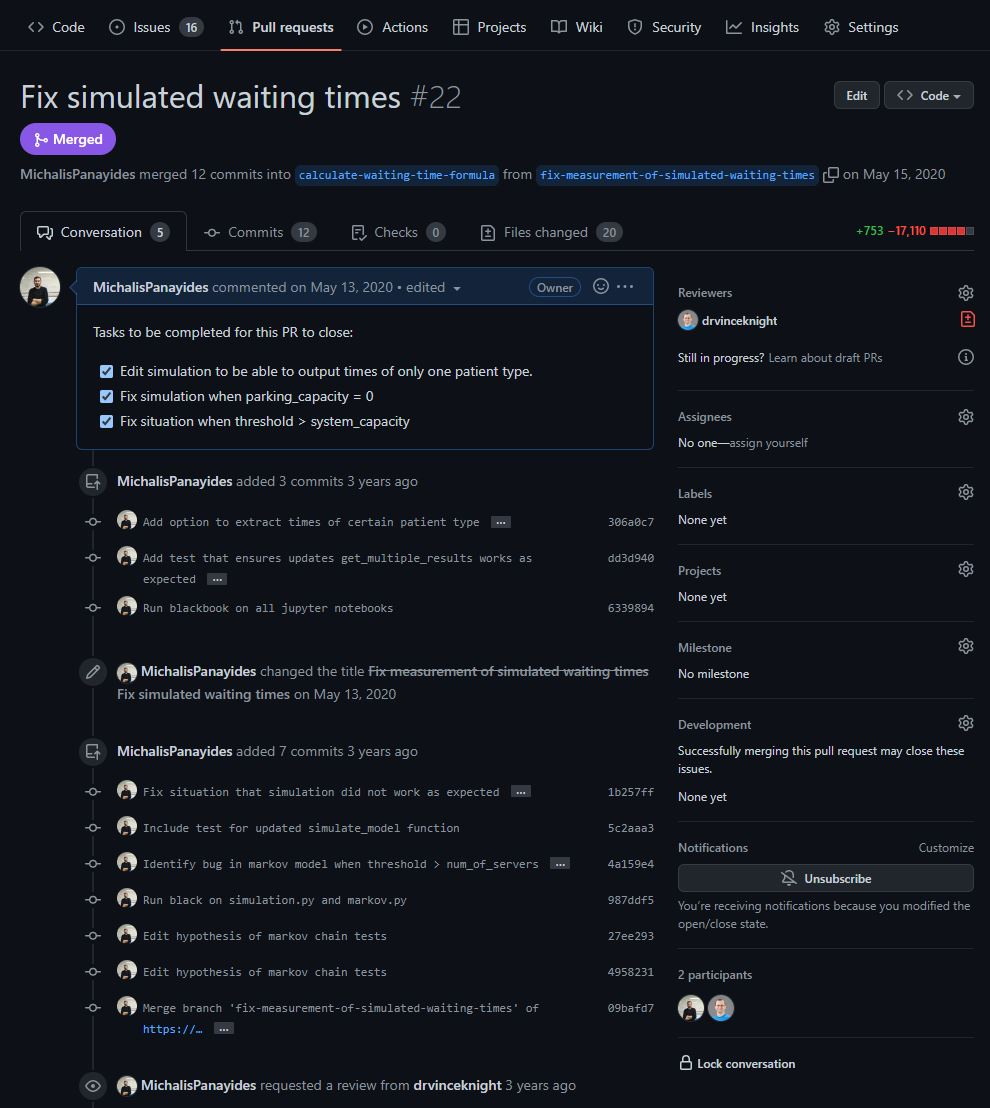
\includegraphics[width=.495\linewidth]{chapters/01_introduction/Bin/commits.JPG}
    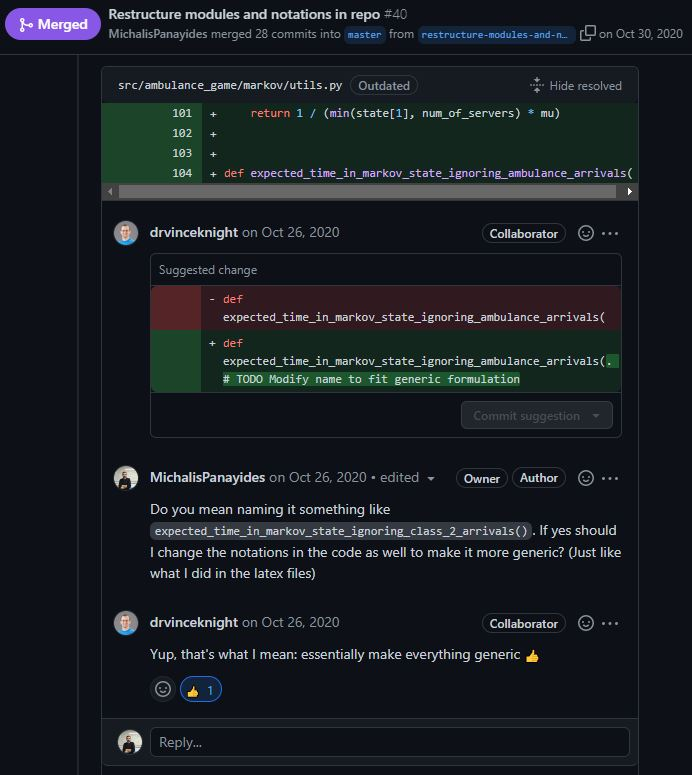
\includegraphics[width=.495\linewidth]{chapters/01_introduction/Bin/conversation.JPG}
    \caption{Pull request example on GitHub.}
    \label{fig:github_pr}
\end{figure}



\subsection{Virtual environments}

A virtual environment is a tool that is used to create an isolated Python
environment on a user's computer for a specific project.
Virtual environments are used to isolate the dependencies of different projects
and to ensure that the dependencies of one project do not interfere with the
dependencies of another project.

There are several tools that can be used for creating virtual environments and
managing dependencies.
For the purposed of this thesis, the \textit{Anaconda} package manager is used.
Anaconda is an open source Python distribution platform that is used for
scientific computing~\cite{rolon2016introduction}.
It offers a number of tools that are used in conjunction with Python.
The most important of these tools is the \textit{Conda} package manager.
Conda is an open source package and environment management system that is used
to install, update and manage packages and their dependencies.
Conda was originally developed for Python programs but it can package and
distribute software for any language.

For every repository that was created for this thesis, a
\textit{conda environment} was created.
Every repository contains a \texttt{.yml} file that contains the list of
dependencies and the versions of the dependencies that are required to run the
software.
The \texttt{.yml} file is recognised by Conda and is used to create the virtual
environment.
Figure~\ref{fig:conda_environment} shows the contents of the \texttt{.yml} file
associated with the repository of this thesis.

\begin{figure}[H]
    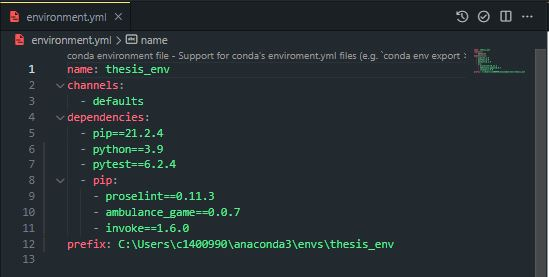
\includegraphics[width=\linewidth]{chapters/01_introduction/Bin/environment.JPG}
    \caption{Conda environment example.}
    \label{fig:conda_environment}
\end{figure}



\subsection{Summary of written software}

The software written for this thesis is written in the open source programming
language Python~\cite{van1995python}.
Python is a general-purpose, object-oriented programming language that is used
for a wide range of applications.
It is both beginner-friendly and powerful with a large community of developers
and users.

For the purposes of this thesis a python library called~\texttt{ambulance\_game}
was developed.
The library contains a number of classes and functions used to formulate and
solve the problem described in this thesis.
More information about the installation and usage of the library can be found
in Appendix~\ref{appendix:ambulance_game}.

One of the most important, and often neglected, aspects of software development
is documentation.
Software documentation is a set of instructions that are used to explain how
software works.
Documentation should explain how users can install and use the software.
All repositories associated with this thesis contain a \texttt{README.md} file
that contains a brief description of the repository and instructions on how to
clone the repository or install the software associated with it.
The source code of the software has been written in a modular and readable
manner with variable and function names that focus on readability.
The source code of the software also contains docstrings that are used to
explain the purpose of the functions and classes created.
Docstrings are a form of documentation that is written directly in the source
code.


\subsection{Testing and code quality checkers}\label{sec:intro_test_code}

Code testing is a process that is used to ensure that the software works as
expected.
A \textit{test} is a piece of code that is used to check the correctness of
another piece of code.
Tests are used to ensure that the software works as expected and that it
produces the correct results.

\begin{quotation}
    ``Testing is the process of executing a program with the intent of finding
    errors.''~\cite{myers2011art}
\end{quotation}


Throughout the development of the software associated with this thesis, a
Test Driven Development (TDD) approach was used.
TDD is a software development process where the tests are written before the
code.
This ensures that all the code is well tested and allows the programmer to
change the program in small steps, increasing overall confidence in the
program's quality~\cite{astels2003test}.

The Python code was tested using the \textit{pytest} library.
Pytest is a testing framework that is used to run tests.
Figure~\ref{fig:test_example} shows an example of a test written that was
written as part of the \texttt{ambulance\_game} library.

\begin{figure}[H]
    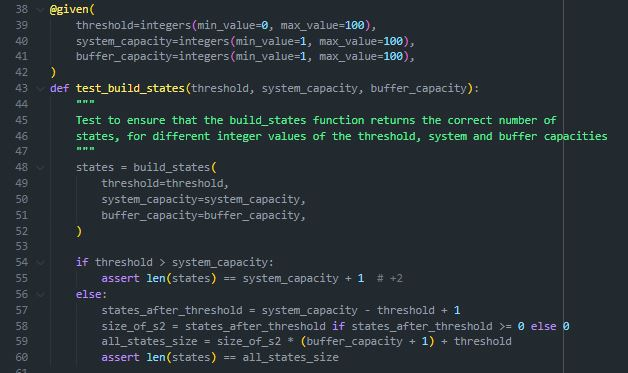
\includegraphics[width=\linewidth]{chapters/01_introduction/Bin/test_example.JPG}
    \caption{Python test example.}
    \label{fig:test_example}
\end{figure}

Apart from testing the code, it is also important to ensure that the code is
well written and that it follows a set of coding standards.
This can be done using a set automated tools that are used to check the code
for common errors and to ensure that the code follows a set of coding standards.
Table~\ref{tab:code_quality_tools} shows a list of tools that were used
throughout the development of software and writing of this thesis.

\begin{table}[H]
    \centering
    \begin{tabular}{|l|l|}
        \hline
        \textbf{Tool} & \textbf{Description} \\
        \hline
        \texttt{black} & A code formatter that is used to ensure that the code
        is \\ & compliant with the PEP8 coding standard~\cite{pep8}. \\
        \hline
        \texttt{flake8} & A tool for style guide enforcement. \\
        \hline
        \texttt{pylint} & A code linter that statically analyses your code. \\
        \hline
        \texttt{mypy} & A Python static type checker. \\
        \hline
        \hline
        \texttt{aspell} & A grammar checker that catches spelling errors. \\
        \hline
        \texttt{alex} & A checker for insensitive and inconsiderate writing. \\
        \hline
        \texttt{proselint} & A linter for prose. \\
        \hline
    \end{tabular}
    \caption{List of tools used to check the code quality.}
    \label{tab:code_quality_tools}
\end{table}

The tools listed in Table~\ref{tab:code_quality_tools} were able to be
automated using the \texttt{tox} library.
Tox is an automation tool that aims to automate and standardise testing in
Python.
It is a generic virtual environment management and test command line tool that
can be used to check if a package installs correctly and run tests.
It also acts as a frontend to Continuous Integration (CI) servers such as
\texttt{GitHub Actions}.
GitHub Actions is a service hosted on GitHub that is used to automate software
development workflows.
It is used to build, test and deploy software.
GitHub Actions was used to automate the testing and code quality checks of the
software associated with this thesis.
Figure~\ref{fig:github_actions} shows an example of a GitHub Actions workflow
that was used to automate the testing and code quality checks of the
\texttt{ambulance\_game} library.

\vspace{1cm}

\begin{figure}[H]
    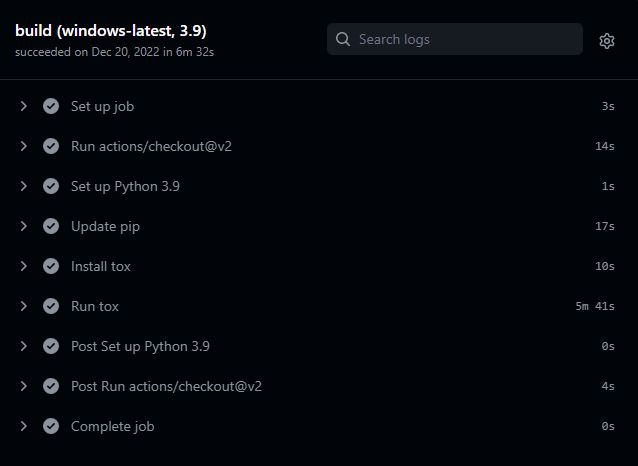
\includegraphics[width=\linewidth]{chapters/01_introduction/Bin/github_actions.JPG}
    \caption{GitHub Actions workflow example.}
    \label{fig:github_actions}
\end{figure}

\newpage
\section{Chapter summary}

This chapter has given an introduction to OR and a brief overview of the
history of OR along with a discussion on queuing theory and game theory.
Additionally, the motivation for the research problem has also been discussed
and the thesis objectives have been defined.

The chapter has also provided an overview of the best practices that were
adopted throughout the development of the software associated with this thesis.
Tools such as tox and GitHub Actions were used to automate the testing
and code quality checks of the software.
